\documentclass[11pt]{article}

\usepackage{iftex}
\ifPDFTeX
\usepackage[T1]{fontenc}
\usepackage[utf8]{inputenc}
\DeclareUnicodeCharacter{2191}{$\uparrow$}
\DeclareUnicodeCharacter{2248}{$\approx$}
\DeclareUnicodeCharacter{2014}{---}
\DeclareUnicodeCharacter{03BC}{$\mu$}
\DeclareUnicodeCharacter{2208}{$\in$}
\DeclareUnicodeCharacter{03BB}{$\lambda$}
\DeclareUnicodeCharacter{21D2}{$\Rightarrow$}
\DeclareUnicodeCharacter{0394}{$\Delta$}
\DeclareUnicodeCharacter{03A9}{$\Omega$}
\DeclareUnicodeCharacter{03A3}{$\Sigma$}
\DeclareUnicodeCharacter{03C1}{$\rho$}
\DeclareUnicodeCharacter{03B5}{$\epsilon$}
\DeclareUnicodeCharacter{2265}{$\geq$}
\else
\usepackage{fontspec}
\fi
\usepackage{amsmath,amssymb,amsthm}
\usepackage{booktabs}
\usepackage{graphicx}
\usepackage[hidelinks]{hyperref}
\usepackage[margin=1in]{geometry}

% Generated by docs/paper/generate_assets.py.
\newcommand{\PaperGeneratedAt}{1970-01-01T00:00:00Z}
\newcommand{\BenchmarkVersion}{0.2.1}
\newcommand{\BenchmarkRepeatCount}{20}
\newcommand{\BenchmarkSystemCount}{15}
\newcommand{\BenchmarkNonWinCount}{9}
\newcommand{\MonteCarloPathCount}{10000}
\newcommand{\MonteCarloHorizon}{200}
\newcommand{\LowerCertificateHorizon}{5}
\newcommand{\VelvetMeasuredCases}{10}


\newtheorem{theorem}{Theorem}
\newtheorem{definition}{Definition}

\title{Max-DE Certified Authorization for Agent Actions}
\author{Paul Chumbe}
% TODO(maintainer): optional affiliation line.
\date{}

\begin{document}
\maketitle

\begin{abstract}
Autonomous agents increasingly propose actions before a human or host system can inspect their consequences. We study certified pre-execution authorization for such actions in a posterior-typed setting. The contribution is a synthesis: computable two-sided decision certificates for action admission, an inspect--lockout--refinement trichotomy, and a formal gap between myopic posterior mean improvement and the martingale supremum value. We implement the certificates in Velvet for Beta--Bernoulli candidates, report the Agent Authorization Benchmark v\BenchmarkVersion{}, and validate the numerical certificate bracket by Monte-Carlo estimates generated from the repository.
\end{abstract}

\section{Problem}

The operational question is not whether an agent can answer a task, but whether a proposed action should be authorized before execution. A pre-execution authority layer must distinguish actions that should proceed, actions that should be blocked, and actions whose value of inspection remains unresolved. It should also leave an artifact that can be replayed, verified, and checked for tampering after the fact.

This paper focuses on posterior-typed action candidates. The canonical example is a Bernoulli arm with unknown success parameter and a host baseline. The action is worth inspecting only if the optionality of future observations clears a price threshold. The benchmark section evaluates the artifact side of this question: certificate emission, determinism across \BenchmarkRepeatCount{} identical runs, replayability, independent verifiability, and tamper-evidence.

\section{System Context}

The repository implements Velvet as a local admission and evidence layer for autonomous-agent actions, with the public surface summarized in \texttt{README.md} and \texttt{IMPLEMENTATION\_STATUS.md}. The admission pipeline takes a typed candidate action, evaluates it through a policy chain, produces an admission decision, and records signed evidence before executable dispatch. On the MCP path, \texttt{docs/mcp\_proxy/evidence.md} describes the proxy evidence artifact as an OAP Decision plus a Velvet-signed Max-DE Certificate Envelope, with ledger records binding request, argument, tool-schema, and policy hashes. The same documentation and \texttt{docs/execution-permits.md} distinguish admission evidence from execution authority: a warrant or proof envelope explains why an action was admitted, while an Execution Permit authorizes one dispatch chain only after the pre-execution record is durable.

Execution Permits are short-lived, single-use authority artifacts bound to the exact request, canonical action, arguments, tool schema, policy hash and version, identity context, audience, signed decision artifact, supporting proof lineage, and durable pre-execution ledger record. Before dispatch, Velvet recomputes the request binding and atomically claims the permit; drift in request, arguments, policy, schema, audience, tenant, environment, or identity context rejects the dispatch. Execution Receipts are signed observations about what the executor or substrate saw after a claimed dispatch, with conservative outcomes such as succeeded, rejected, failed before dispatch, or indeterminate. The receipt contract is deliberately weaker than a business-level side-effect proof; \texttt{docs/execution-permits.md} states that a gateway-observed receipt proves gateway observation rather than final business outcome.

The Vault evidence plane extends ledger records with RFC-6962-style Merkle roots over ordered record hashes, Signed Tree Heads, inclusion proofs, consistency proofs, anchor receipts, and retention tombstones as documented in \texttt{docs/vault.md}. Verification recomputes frame hashes, record hashes, semantic chain links, Merkle roots, inclusion proofs, Signed Tree Head signatures, and optional consistency against a previous tree head. Consistency proofs and single-use execution authority are strictly stronger evidence structures than an append-only hash chain alone because a verifier can check both record inclusion in a signed tree and tree growth between checkpoints, while the permit claim path rejects reuse before dispatch.

\section{Formal Model}

Let $\theta \sim \mathrm{Beta}(\alpha,\beta)$ and fix a baseline $v \in (0,1)$. Define the posterior improvement payoff
\[
    Y=(\theta-v)^+.
\]
Let $(\mathcal{F}_n)_{n\geq 0}$ be the filtration generated by hypothetically sampling the same Bernoulli arm and let
\[
    M_n=\mathbb{E}[Y\mid \mathcal{F}_n].
\]
The Max-DE value is the martingale-supremum value
\[
    \Phi_v(\alpha,\beta)=\mathbb{E}\left[\sup_{n\geq 0} M_n\right].
\]
The myopic posterior expected improvement is only $M_0$. The gap $\Phi_v-M_0$ is the pick-me mass: the value of future posterior paths that may make an action admissible even when the current posterior mean improvement is below price.

Given a delight scale $L$ and action price $\lambda$, write $c=\lambda/L$. The implementation computes a lower certificate $L_v^{(r)}(\alpha,\beta)$ and an upper certificate $U_v(\alpha,\beta)$ from \texttt{src/velvet/research/bernoulli.py}. The admission rule is:
\[
\begin{array}{ll}
\text{inspect} & \text{if } L_v^{(r)}(\alpha,\beta)\geq c,\\
\text{lockout} & \text{if } U_v(\alpha,\beta)<c,\\
\text{refine} & \text{otherwise.}
\end{array}
\]

\section{Certificates and Proof Sources}

The proof ingredients are classical. Ville's inequality gives the logarithmic maximal envelope, Doob's $L^2$ maximal inequality gives the quadratic envelope, and the layer-cake/Markov-chain hitting argument gives the exact supremum representation. The contribution here is not those tools; it is the computable synthesis into a two-sided certificate interface for action admission.

\begin{theorem}[Two-sided certified gate]
For each finite horizon $r$, the generated lower certificate and production upper certificate satisfy
\[
    L_v^{(r)}(\alpha,\beta)\leq \Phi_v(\alpha,\beta)\leq U_v(\alpha,\beta).
\]
Therefore the inspect and lockout branches above are sound, while the remaining region is a refinement zone rather than evidence for permanent rejection.
\end{theorem}

The theorem and supporting notes are transcribed verbatim from the eight files in \texttt{docs/math/} in Appendix~\ref{app:proofs}. The generated source audit records the SHA-256 of each proof source and of \texttt{src/velvet/research/bernoulli.py}.

\section{Empirical Artifact Benchmark}

The Agent Authorization Benchmark v\BenchmarkVersion{} contains \BenchmarkSystemCount{} seeded system rows. It is generated from the repository's liability benchmark adapters plus Velvet replay and signing checks. Not-run entries identify missing packages or credentials and are not treated as competitor failures. The pass\textsuperscript{k} reliability reporting follows tau-bench~(\href{https://arxiv.org/abs/2406.12045}{arXiv:2406.12045}), estimating the probability that all sampled repeated runs are successful; PolicyGuard~(\href{https://arxiv.org/abs/2606.32004}{arXiv:2606.32004}) applies the same estimator to document-compliance policy review.

\begin{center}
\small
\begin{tabular}{lccccc}
\toprule
System & Cert. & Det. & Replay & Public verify & Tamper \\
\midrule
Amazon Bedrock Guardrails & NR & NR & NR & NR & NR \\
Azure AI Content Safety & NR & NR & NR & NR & NR \\
Guardrails AI & NR & NR & NR & NR & NR \\
Lakera Guard & NR & NR & NR & NR & NR \\
NVIDIA NeMo Guardrails & NR & NR & NR & NR & NR \\
OpenAI Agents SDK guardrails & NR & NR & NR & NR & NR \\
Velvet Certified Max-DE & Y & Y & Y & Y & Y \\
epsilon\_greedy & N & Y & N & N & N \\
final\_output\_guardrail & N & Y & N & N & N \\
human\_review\_queue & N & Y & N & N & N \\
mcp\_allowlist\_only & N & Y & N & N & N \\
myopic\_delight\_gate & N & Y & N & N & N \\
prompt\_only\_policy & N & Y & N & N & N \\
thompson\_sampling & N & N & N & N & N \\
ucb\_fixed\_threshold & N & Y & N & N & N \\
\bottomrule
\end{tabular}

\end{center}

Velvet does not win every seeded liability-cost row. The generated non-win table records \BenchmarkNonWinCount{} rows where another local baseline matches or beats Velvet on the benchmark cost scalar while lacking the certificate/seal evidence measured above.

\begin{center}
\scriptsize
\begin{tabular}{ll}
\toprule
Case & Matching or lower benchmark liability cost \\
\midrule
air\_canada\_chatbot\_policy\_liability\_2024 & human\_review\_queue (defer\_for\_review, cost=0.0) \\
certifiable\_waste\_beta\_1\_3 & myopic\_delight\_gate (skip\_without\_certificate, cost=0.0) \\
dpd\_prompt\_policy\_bypass\_2024 & human\_review\_queue (defer\_for\_review, cost=0.0) \\
nyc\_mycity\_illegal\_business\_advice\_2024 & human\_review\_queue (defer\_for\_review, cost=0.0) \\
replit\_production\_database\_deletion\_2025 & human\_review\_queue (defer\_for\_review, cost=0.0) \\
tau\_airline\_book\_reservation\_0 & human\_review\_queue (defer\_for\_review, cost=0.0) \\
tau\_airline\_cancel\_reservation\_1 & human\_review\_queue (defer\_for\_review, cost=0.0) \\
tau\_retail\_exchange\_delivered\_order\_0 & human\_review\_queue (defer\_for\_review, cost=0.0) \\
tau\_retail\_return\_delivered\_order\_2 & human\_review\_queue (defer\_for\_review, cost=0.0) \\
\bottomrule
\end{tabular}

\end{center}

\section{Numerical Certificate Validation}

The figure and table below are generated by \texttt{docs/paper/generate\_assets.py}. For each Beta--Bernoulli setting, the script computes the analytic lower certificate with horizon \LowerCertificateHorizon{}, the production upper certificate from \texttt{src/velvet/research/bernoulli.py}, and a Monte-Carlo estimate $\hat{\Phi}$ using \MonteCarloPathCount{} posterior-predictive paths of horizon \MonteCarloHorizon{} with fixed seeds. The generated script fails if any point estimate falls outside its certificate bracket.

\begin{figure}[h]
    \centering
    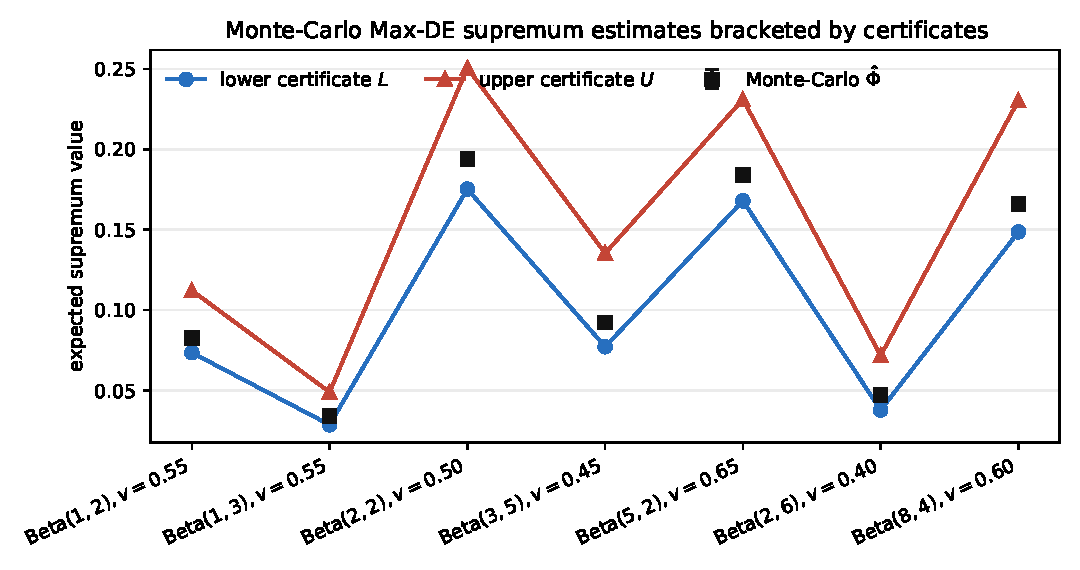
\includegraphics[width=\linewidth]{figures/mc_bounds.pdf}
    \caption{Repository-generated Monte-Carlo estimates of the Max-DE martingale-supremum value bracketed by analytic lower and upper certificates.}
\end{figure}

\begin{center}
\small
\begin{tabular}{rrrrrrr}
\toprule
$\alpha$ & $\beta$ & $v$ & $L^{(5)}$ & $\hat{\Phi}$ & 95\% half-width & $U$ \\
\midrule
1 & 2 & 0.55 & 0.0736 & 0.0827 & 0.0016 & 0.1123 \\
1 & 3 & 0.55 & 0.0287 & 0.0343 & 0.0010 & 0.0490 \\
2 & 2 & 0.50 & 0.1753 & 0.1940 & 0.0020 & 0.2507 \\
3 & 5 & 0.45 & 0.0773 & 0.0922 & 0.0014 & 0.1354 \\
5 & 2 & 0.65 & 0.1680 & 0.1841 & 0.0013 & 0.2310 \\
2 & 6 & 0.40 & 0.0378 & 0.0474 & 0.0011 & 0.0718 \\
8 & 4 & 0.60 & 0.1487 & 0.1659 & 0.0012 & 0.2304 \\
\bottomrule
\end{tabular}

\end{center}

\section{Limitations}

The formal certificates in this paper apply to posterior-typed Bernoulli candidates. They do not certify arbitrary tool calls, arbitrary code execution, model truthfulness, or production compliance. The Agent Authorization Benchmark measures authorization artifacts rather than end-task success. External adapters in the seeded run are not live provider evaluations when optional packages or credentials are absent. HMAC signatures remain local-dev only and are not used for independent public verification claims.

The Monte-Carlo validation is numerical evidence against transcription and implementation mistakes, not a replacement for the analytic proof. The estimate uses a large finite horizon and terminal payoff sample; the certificate comparison is the rigorous object.

\section{Reproducibility}

The paper assets are generated from repository files, not hand-entered benchmark or figure values. The relevant commands are:

\begin{verbatim}
uv run velvet agent-auth-benchmark --report-dir reports/agent_auth
uv run python docs/paper/generate_assets.py
uv run python docs/paper/build.py
uv run pytest
uv run ruff check .
uv run mypy src tests
cargo fmt --check
cargo clippy --workspace --all-targets -- -D warnings
cargo test --workspace
\end{verbatim}


The benchmark package is under \texttt{benchmarks/agent\_authorization/}. The seal-conformance suite is \texttt{tests/test\_seal\_conformance.py}. The generated audit file is \texttt{docs/paper/generated/source\_audit.json}.

\appendix
% Generated verbatim from docs/math/*.txt by docs/paper/generate_assets.py.
\section{Verbatim Proof Source Notes}
\label{app:proofs}
The following source notes are included verbatim from the repository. They are not retyped in this paper.
\subsection{exact max de theorem}
\begin{small}
\begin{verbatim}
Exact Max-DE as a Beta-Bernoulli Martingale Hitting Problem

Theorem.

Let alpha,beta > 0 and v in (0,1). Let

    Theta ~ Beta(alpha,beta).

Conditional on Theta = theta, let

    X_1, X_2, ... | Theta = theta  iid~  Bernoulli(theta).

Define

    S_n = sum_{i=1}^n X_i,
    R_n = n - S_n,
    F_n = sigma(X_1,...,X_n),

where F_n denotes the observation filtration. Let

    Y = (Theta - v)^+.

For a,b > 0, define the Beta-Bernoulli expected-improvement functional

    g_v(a,b)
    =
    E_{theta ~ Beta(a,b)}[(theta - v)^+].

Equivalently,

    g_v(a,b)
    =
    integral_v^1 (theta - v)
        theta^{a-1}(1-theta)^{b-1} / B(a,b)
    dtheta.

In incomplete-beta notation,

    g_v(a,b)
    =
    a/(a+b) * (1 - I_v(a+1,b))
    -
    v * (1 - I_v(a,b)).

Define the posterior expected-improvement process

    M_n = E[Y | F_n].

Then

    M_n = g_v(alpha + S_n, beta + R_n).

The exact Max-DE value is

    D^max(alpha,beta;v)
    =
    L E[sup_{n >= 0} M_n].

Then the following hold.

1. Martingale structure.

The process (M_n)_{n >= 0} is a bounded uniformly integrable Doob martingale. More precisely,

    0 <= M_n <= 1 - v

almost surely for every n, and

    E[M_{n+1} | F_n] = M_n.

Moreover,

    M_n -> Y = (Theta - v)^+

almost surely and in L^1.

Proof.

Since

    0 <= Y <= 1 - v,

we have Y in L^\infty. Therefore

    M_n = E[Y | F_n]

is an integrable adapted process, and by the tower property,

    E[M_{n+1} | F_n]
    =
    E[E[Y | F_{n+1}] | F_n]
    =
    E[Y | F_n]
    =
    M_n.

Also, conditional expectation preserves order, so

    0 <= M_n <= 1 - v.

Thus (M_n) is bounded in L^\infty and hence uniformly integrable.

By martingale convergence, M_n converges almost surely and in L^1 to

    M_infty = E[Y | F_infty],

where

    F_infty = sigma(union_n F_n).

Under the Beta-Bernoulli construction,

    S_n / n -> Theta

almost surely. Hence Theta is F_infty-measurable, so Y is F_infty-measurable, and therefore

    M_infty = E[Y | F_infty] = Y.

This proves the martingale claim.


2. Exact layer-cake representation.

Let

    Z = sup_{n >= 0} M_n.

Since 0 <= Z <= 1 - v, the layer-cake formula gives

    E[Z]
    =
    integral_0^{1-v} P(Z >= x) dx.

For x in [0,1-v], define

    h_x(a,b)
    =
    P_{a,b}(exists n >= 0 :
        g_v(a + S_n, b + R_n) >= x).

Then

    E[sup_{n >= 0} M_n]
    =
    integral_0^{1-v} h_x(alpha,beta) dx.

Consequently,

    D^max(alpha,beta;v)
    =
    L integral_0^{1-v} h_x(alpha,beta) dx.

Proof.

Because Z is the countable supremum of measurable random variables, Z is measurable. Since it is bounded and nonnegative,

    E[Z]
    =
    integral_0^{1-v} P(Z >= x) dx.

Now

    Z >= x

if and only if

    exists n >= 0 such that M_n >= x.

Using

    M_n = g_v(alpha + S_n, beta + R_n),

we obtain

    P(Z >= x)
    =
    P_{alpha,beta}(exists n >= 0 :
        g_v(alpha + S_n, beta + R_n) >= x)
    =
    h_x(alpha,beta).

Substitution into the layer-cake identity gives the result.


3. Posterior-lattice hitting formulation.

For fixed x in (0,1-v), define the posterior lattice

    L_{a,b}
    =
    {(a+i,b+j): i,j in N_0}.

Define the posterior-state Markov chain

    (A_n,B_n) = (a + S_n, b + R_n).

Its transition kernel is

    (a,b) -> (a+1,b) with probability a/(a+b),

and

    (a,b) -> (a,b+1) with probability b/(a+b).

Define the hitting set

    G_x = {(a,b): g_v(a,b) >= x},

and the hitting time

    tau_x = inf{n >= 0 : (A_n,B_n) in G_x}.

Then

    h_x(a,b) = P_{a,b}(tau_x < infinity).

Furthermore, h_x satisfies the Dirichlet problem

    h_x(a,b) = 1
    if (a,b) in G_x,

and, if (a,b) notin G_x,

    h_x(a,b)
    =
    a/(a+b) h_x(a+1,b)
    +
    b/(a+b) h_x(a,b+1).

Proof.

The posterior predictive probability of success from state (a,b) is

    E[Theta | A_n=a, B_n=b] = a/(a+b),

and the predictive probability of failure is b/(a+b). Hence (A_n,B_n) is the stated Markov chain.

By definition, the event

    tau_x < infinity

is exactly the event that the process ever reaches a state where

    g_v(A_n,B_n) >= x.

Therefore

    h_x(a,b) = P_{a,b}(tau_x < infinity).

If (a,b) in G_x, then tau_x = 0, so h_x(a,b)=1.

If (a,b) notin G_x, first-step analysis and the Markov property give

    h_x(a,b)
    =
    a/(a+b) h_x(a+1,b)
    +
    b/(a+b) h_x(a,b+1).

This proves the harmonic recursion.


4. Minimality and boundary at infinity.

The function h_x is the minimal nonnegative solution of the above Dirichlet problem.

That is, if u >= 0 satisfies

    u(a,b) = 1
    on G_x,

and

    u(a,b)
    =
    a/(a+b) u(a+1,b)
    +
    b/(a+b) u(a,b+1)

on G_x^c, then

    h_x(a,b) <= u(a,b)

for every lattice state (a,b).

Equivalently,

    h_x(a,b)
    =
    lim_{N -> infinity} h_x^{(N)}(a,b),

where

    h_x^{(N)}(a,b)
    =
    P_{a,b}(tau_x <= N).

The finite-horizon approximants satisfy

    h_x^{(0)}(a,b) = 1_{g_v(a,b) >= x},

and recursively,

    h_x^{(N+1)}(a,b) = 1
    on G_x,

while outside G_x,

    h_x^{(N+1)}(a,b)
    =
    a/(a+b) h_x^{(N)}(a+1,b)
    +
    b/(a+b) h_x^{(N)}(a,b+1).

Moreover,

    h_x^{(N)}(a,b) increases to h_x(a,b).

Proof.

Let u be any nonnegative solution with boundary value 1 on G_x. Let tau = tau_x. For finite N, harmonicity before hitting G_x and constancy after hitting G_x imply

    u(a,b)
    =
    E_{a,b}[u(A_{N wedge tau}, B_{N wedge tau})].

On the event {tau <= N}, the stopped chain lies in G_x, so the stopped value is 1. On the event {tau > N}, nonnegativity gives a contribution at least 0. Therefore

    u(a,b)
    >=
    P_{a,b}(tau <= N).

Letting N -> infinity yields

    u(a,b)
    >=
    P_{a,b}(tau < infinity)
    =
    h_x(a,b).

Thus h_x is minimal.

The finite-horizon formula follows from the same first-step recursion and the monotone convergence of the events

    {tau_x <= N} increasing to {tau_x < infinity}.

This minimality condition is the correct boundary condition at infinity. The chain has no finite absorbing boundary except G_x; it moves forever toward larger a+b. Paths that escape to infinity without hitting G_x contribute zero to the hitting probability.


5. Boundary conditions.

For x <= 0,

    h_x(a,b) = 1.

For x > 1 - v,

    h_x(a,b) = 0.

For finite a,b and x = 1 - v,

    h_{1-v}(a,b) = 0,

because g_v(a,b) < 1 - v at every finite posterior state.

For x in (0,1-v),

    h_x(a,b) = 1
    whenever g_v(a,b) >= x.

There is no boundary at a=0 or b=0, because alpha,beta > 0 and the posterior lattice only moves by increasing one coordinate. The only nontrivial boundary data are:

    h_x = 1 on G_x,

together with the minimality condition at infinity.


6. Exactness and non-O(1) nature.

The representation

    D^max(alpha,beta;v)
    =
    L integral_0^{1-v} h_x(alpha,beta) dx

is exact because it follows from:

    (i) the Doob martingale identity M_n = E[Y | F_n];

    (ii) the equivalence between {sup_n M_n >= x} and hitting the posterior-lattice set G_x;

    (iii) the layer-cake formula for bounded nonnegative random variables.

However, this is not generally an O(1) algebraic closed form.

The local function g_v(a,b) is O(1)-computable through incomplete beta functions. But h_x(a,b) is an infinite-horizon first-passage probability for a nonhomogeneous Markov chain on an infinite lattice. The boundary

    g_v(a,b) = x

is generally nonlinear and depends on incomplete beta functions. Thus the event

    exists n >= 0 : g_v(A_n,B_n) >= x

is genuinely path-dependent.

Beta-binomial identities give fixed-time probabilities such as

    P_{a,b}(S_n=s)
    =
    binomial(n,s) B(a+s,b+n-s) / B(a,b),

and hence can compute

    P_{a,b}(M_n >= x)

for fixed n. But they do not eliminate the first-passage condition

    P_{a,b}(exists n >= 0 : M_n >= x).

Therefore standard potential theory and Markov chain hitting theory give the exact characterization, finite-horizon approximations, and bounds, but not a general O(1) algebraic formula.


7. Useful sharp bounds.

Since

    M_n -> Y = (Theta - v)^+

almost surely, the event {Y > x} implies eventual crossing of level x. Hence, for 0 < x < 1-v,

    h_x(a,b)
    >=
    P_{Theta ~ Beta(a,b)}(Theta > v+x)
    =
    1 - I_{v+x}(a,b).

On the other hand, since (M_n) is a nonnegative martingale, Ville's inequality gives

    h_x(a,b)
    =
    P_{a,b}(sup_n M_n >= x)
    <=
    min{1, g_v(a,b)/x}.

Therefore, for 0 < x < 1-v,

    1 - I_{v+x}(a,b)
    <=
    h_x(a,b)
    <=
    min{1, g_v(a,b)/x}.

These bounds identify the exact object as lying between terminal realized upside and the martingale maximal envelope.


Final exact statement.

The exact Max-DE value for a Beta-Bernoulli arm is

    D^max(alpha,beta;v)
    =
    L integral_0^{1-v}
        P_{alpha,beta}(
            exists n >= 0 :
            g_v(alpha + S_n, beta + R_n) >= x
        )
    dx.

Equivalently,

    D^max(alpha,beta;v)
    =
    L integral_0^{1-v} h_x(alpha,beta) dx,

where h_x is the minimal nonnegative solution of

    h_x(a,b) = 1
    if g_v(a,b) >= x,

and otherwise

    h_x(a,b)
    =
    a/(a+b) h_x(a+1,b)
    +
    b/(a+b) h_x(a,b+1).

Thus Max-DE is exactly the layer-cake integral of posterior-martingale first-passage probabilities on the Beta-Bernoulli lattice.
\end{verbatim}
\end{small}
\subsection{lower certificates for max de inspection theorem}
\begin{small}
\begin{verbatim}
Lower Certificates for Max-DE Inspection

Setup.
Let theta ~ Beta(alpha,beta), with alpha,beta > 0, and fix v in (0,1). Define

    Y = (theta - v)^+,

and let (F_n) be the posterior filtration generated by hypothetically sampling the same Bernoulli arm n additional times. Define

    M_n = E[Y | F_n]
        = g_v(alpha + S_n, beta + F_n),

where

    g_v(a,b) = E_{theta ~ Beta(a,b)}[(theta - v)^+].

The exact Max-DE value is

    Phi_v(alpha,beta) = E[sup_{n >= 0} M_n].

The expected-improvement functional has the computable form

    g_w(a,b)
    =
    a/(a+b) * [1 - I_w(a+1,b)]
    -
    w * [1 - I_w(a,b)],

for 0 <= w < 1, where I_w(a,b) is the regularized incomplete beta function. Set g_w(a,b)=0 for w >= 1.

Theorem.
For every integer r >= 0, define the terminal-augmented finite-horizon lower certificate

    L^+_{v,r}(alpha,beta)
    =
    E[max{Y, M_0, M_1, ..., M_r}].

Then:

    g_v(alpha,beta)
    <=
    L^+_{v,0}(alpha,beta)
    <=
    L^+_{v,1}(alpha,beta)
    <=
    ...
    <=
    Phi_v(alpha,beta).

Moreover,

    L^+_{v,r}(alpha,beta) ↑ Phi_v(alpha,beta)
    as r -> infinity.

Thus L^+_{v,r} is a certified, monotone, computable lower approximation to the exact Max-DE value.

Proof.
Since 0 <= Y <= 1-v, the process

    M_n = E[Y | F_n]

is a bounded uniformly integrable Doob martingale. In the Beta-Bernoulli model, the infinite hypothetical sample path identifies theta almost surely through the empirical mean, so the posterior concentrates at theta and

    M_n -> Y almost surely.

Therefore

    max{Y, M_0, ..., M_r} <= sup_{n >= 0} M_n

for every finite r, and hence

    L^+_{v,r}(alpha,beta) <= Phi_v(alpha,beta).

The sequence is monotone in r because each additional lookahead term only enlarges the maximum. Since M_n -> Y almost surely,

    max{Y, M_0, ..., M_r} ↑ sup_{n >= 0} M_n.

Monotone convergence gives

    L^+_{v,r}(alpha,beta) ↑ E[sup_{n >= 0} M_n]
    =
    Phi_v(alpha,beta).

This proves the theorem.

Recursive computation.
For a posterior state (a,b) and running maximum z, define

    B_0(a,b,z) = z + g_{v+z}(a,b).

For r >= 0, define recursively

    B_{r+1}(a,b,z)
    =
    a/(a+b) *
    B_r(a+1,b, max{z, g_v(a+1,b)})
    +
    b/(a+b) *
    B_r(a,b+1, max{z, g_v(a,b+1)}).

Then

    L^+_{v,r}(alpha,beta)
    =
    B_r(alpha,beta, g_v(alpha,beta)).

This recursion is exact for fixed r.

Proof of recursion.
At state (a,b), the next predictive success probability is a/(a+b), and the next predictive failure probability is b/(a+b). A success moves the posterior to (a+1,b), while a failure moves it to (a,b+1). The running maximum z updates to

    max{z, g_v(a+1,b)}

after success, and to

    max{z, g_v(a,b+1)}

after failure.

At terminal depth, conditional on posterior state (a,b),

    E[max{z,Y}]
    =
    z + E[(Y-z)^+]
    =
    z + E[((theta-v)^+ - z)^+]
    =
    z + E[(theta - v - z)^+]
    =
    z + g_{v+z}(a,b).

This gives the recursion.

Zero-step closed certificate.
Let

    m_v = g_v(alpha,beta).

Then

    L^+_{v,0}(alpha,beta)
    =
    E[max{Y,m_v}]
    =
    m_v + g_{v+m_v}(alpha,beta).

This strictly improves the trivial lower bound Phi_v >= m_v whenever v+m_v < 1.

One-step certificate.
Let

    m  = g_v(alpha,beta),
    mS = g_v(alpha+1,beta),
    mF = g_v(alpha,beta+1),
    p  = alpha/(alpha+beta).

Then

    L^+_{v,1}(alpha,beta)
    =
    p  * [zS + g_{v+zS}(alpha+1,beta)]
    +
    (1-p) * [zF + g_{v+zF}(alpha,beta+1)],

where

    zS = max{m,mS},
    zF = max{m,mF}.

For the monotone payoff (theta-v)^+, usually mS >= m >= mF, so this reduces to

    L^+_{v,1}(alpha,beta)
    =
    p  * [mS + g_{v+mS}(alpha+1,beta)]
    +
    (1-p) * [m + g_{v+m}(alpha,beta+1)].

Specialization: Beta(1,2).
Let theta ~ Beta(1,2) and set c = 1-v. Then

    g_v(1,2) = c^3/3,

    g_v(2,2) = c^3(1+v)/2,

    g_v(1,3) = c^4/4.

The zero-step certificate is

    L^+_{v,0}(1,2)
    =
    c^3/3
    +
    (c - c^3/3)^3 / 3.

The one-step certificate is

    L^+_{v,1}(1,2)
    =
    1/3 * [g_v(2,2) + g_{v+g_v(2,2)}(2,2)]
    +
    2/3 * [g_v(1,2) + g_{v+g_v(1,2)}(1,3)].

For v=0.5, one obtains

    g_v(1,2)                 = 0.0416667,
    L^+_{v,0}(1,2)           ≈ 0.0737606,
    L^+_{v,1}(1,2)           ≈ 0.0841920,
    L^+_{v,2}(1,2)           ≈ 0.0886848,
    L^+_{v,3}(1,2)           ≈ 0.0920982.

Thus, in the canonical tried-better-arm trap,

    Phi_{0.5}(1,2) >= 0.0920982

using only a three-step certified lower certificate, more than twice the myopic expected improvement 0.0416667.

Certified inspection / lockout rule.
Let

    q = lambda / L.

Let ell_v(alpha,beta) be any certified lower bound, for example

    ell_v(alpha,beta) = L^+_{v,r}(alpha,beta),

and let U_v(alpha,beta) be any rigorous upper certificate satisfying

    Phi_v(alpha,beta) <= U_v(alpha,beta).

Then the production decision rule is:

    if ell_v(alpha,beta) >= q:
        inspect

    elif U_v(alpha,beta) < q:
        lock out

    else:
        unresolved band.

Equivalently, in original delight units:

    if L * ell_v(alpha,beta) >= lambda:
        inspect

    elif L * U_v(alpha,beta) < lambda:
        lock out

    else:
        unresolved band.

The normalized unresolved-band width is

    U_v(alpha,beta) - ell_v(alpha,beta),

and the original delight-scale width is

    L * [U_v(alpha,beta) - ell_v(alpha,beta)].

Corollary with the Ville/log upper certificate.
If the upper certificate is chosen as

    U_log,v(alpha,beta)
    =
    min{
        1-v,
        m_v * [1 + log((1-v)/m_v)]
    },

with m_v = g_v(alpha,beta), then for Beta(1,2), v=0.5,

    0.0920982 <= Phi_{0.5}(1,2) <= 0.14520.

Therefore, for the normalized threshold q=lambda/L,

    q <= 0.0920982       implies certified inspection,
    q >  0.14520         implies certified lockout,
    0.0920982 < q <= 0.14520 implies unresolved.

Main conclusion.
The terminal-augmented finite-horizon certificate

    L^+_{v,r}(alpha,beta)
    =
    E[max{Y, M_0, ..., M_r}]

is the clean lower-certificate counterpart to the existing upper safe-lockout certificates. It is rigorous, monotone, convergent, computable for general Beta(alpha,beta), and already strong for small r. For production, r=3 is a natural default inspection certificate.
\end{verbatim}
\end{small}
\subsection{O1 Martingale Maximal Certificates for Safe Lockout}
\begin{small}
\begin{verbatim}
O(1) Martingale Maximal Certificates for Safe Lockout
========================================================

Theorem.
--------

Let

    Y = (theta - v)^+,

where

    theta ~ Beta(alpha, beta),
    alpha > 0,
    beta > 0,
    v in (0,1).

Let (F_n)_{n >= 0} be the posterior filtration generated by hypothetically sampling the same Bernoulli arm n additional times, and define

    M_n = E[Y | F_n].

Set

    m_v = E[Y],
    s_v = E[Y^2],
    c_v = 1 - v.

Then (M_n)_{n >= 0} is a bounded uniformly integrable Doob martingale satisfying

    0 <= M_n <= c_v

for every n. If

    M^* = sup_{n >= 0} M_n,

then

    E[M^*] <= U_prod,v^+(alpha,beta),

where

    U_prod,v^+(alpha,beta)
    =
    min{
        c_v,
        U_log,v(alpha,beta),
        U_2,+,v(alpha,beta)
    },

with

    U_log,v(alpha,beta)
    =
    min{
        c_v,
        m_v [1 + log(c_v / m_v)]
    },

using the convention that the logarithmic term is 0 when m_v = 0, and

    U_2,+,v(alpha,beta)
    =
    min{
        c_v,
        m_v + 2 sqrt(q_v)
    },

where

    q_v = E[(Y - m_v)_+^2].

Consequently, the coarser but simpler certificate

    U_prod,v(alpha,beta)
    =
    min{
        c_v,
        U_log,v(alpha,beta),
        m_v + 2 sqrt(s_v - m_v^2)
    }

is also valid, since

    q_v <= s_v - m_v^2.

Thus

    E[sup_{n >= 0} M_n]
    <=
    U_prod,v^+(alpha,beta)
    <=
    U_prod,v(alpha,beta).

These are rigorous O(1) upper certificates. They are not exact formulas for the Max-DE price.


Proof.
------

1. Martingale structure.

Since

    M_n = E[Y | F_n],

(M_n) is the Doob martingale associated with the terminal bounded random variable Y. Because

    0 <= Y <= 1 - v = c_v,

conditional expectation gives

    0 <= M_n <= c_v

for every n. Hence (M_n) is bounded and therefore uniformly integrable.

Let

    M^* = sup_{n >= 0} M_n.

Then

    0 <= M^* <= c_v.


2. Ville/log envelope.

Since (M_n) is a nonnegative martingale with

    M_0 = E[Y] = m_v,

Ville's inequality gives, for every finite horizon N and every x > 0,

    P(max_{0 <= n <= N} M_n >= x) <= m_v / x.

Letting N -> infinity yields

    P(M^* >= x) <= m_v / x.

Since probabilities are at most 1,

    P(M^* >= x) <= min{1, m_v / x}.

By the layer-cake formula,

    E[M^*]
    =
    integral_0^{c_v} P(M^* >= x) dx.

Therefore, if m_v > 0,

    E[M^*]
    <=
    integral_0^{c_v} min{1, m_v / x} dx
    =
    integral_0^{m_v} 1 dx
    +
    integral_{m_v}^{c_v} (m_v / x) dx
    =
    m_v + m_v log(c_v / m_v).

Thus

    E[M^*]
    <=
    m_v [1 + log(c_v / m_v)].

Together with the trivial bound M^* <= c_v,

    E[M^*] <= U_log,v(alpha,beta).

If m_v = 0, then Y = 0 almost surely, hence M_n = 0 almost surely for every n, so E[M^*] = 0. This justifies the stated convention.


3. Symmetric Doob L^2 envelope.

Define the centred martingale

    N_n = M_n - m_v.

Then N_0 = 0. For each finite horizon N,

    max_{0 <= n <= N} M_n
    =
    m_v + max_{0 <= n <= N} N_n
    <=
    m_v + max_{0 <= n <= N} |N_n|.

Taking expectations, applying Cauchy-Schwarz, and then Doob's L^2 maximal inequality,

    E[max_{0 <= n <= N} M_n]
    <=
    m_v
    +
    E[max_{0 <= n <= N} |N_n|]
    <=
    m_v
    +
    (E[max_{0 <= n <= N} |N_n|^2])^{1/2}
    <=
    m_v
    +
    2 (E[N_N^2])^{1/2}.

Now

    N_N = E[Y | F_N] - E[Y].

By L^2 contraction of conditional expectation,

    E[N_N^2]
    =
    Var(E[Y | F_N])
    <=
    Var(Y)
    =
    s_v - m_v^2.

Therefore

    E[max_{0 <= n <= N} M_n]
    <=
    m_v + 2 sqrt(s_v - m_v^2).

Letting N -> infinity by monotone convergence,

    E[M^*]
    <=
    m_v + 2 sqrt(s_v - m_v^2).

Together with M^* <= c_v, this proves the symmetric L^2 certificate.


4. Sharper one-sided Doob L^2 envelope.

The symmetric certificate is valid but wasteful because Max-DE only prices upward optionality.

Again let

    N_n = M_n - m_v.

Since N_0 = 0,

    sup_{0 <= n <= N} M_n
    =
    m_v + sup_{0 <= n <= N} N_n
    =
    m_v + sup_{0 <= n <= N} N_n^+.

The process N_n^+ is a nonnegative submartingale. Doob's L^2 inequality applied to N_n^+ gives

    E[sup_{0 <= n <= N} (N_n^+)^2]
    <=
    4 E[(N_N^+)^2].

Therefore

    E[sup_{0 <= n <= N} N_n^+]
    <=
    2 sqrt(E[(N_N^+)^2]).

Since

    N_N
    =
    E[Y - m_v | F_N],

conditional Jensen gives

    (N_N^+)^2
    =
    (E[Y - m_v | F_N]^+)^2
    <=
    E[(Y - m_v)_+^2 | F_N].

Thus

    E[(N_N^+)^2]
    <=
    E[(Y - m_v)_+^2]
    =
    q_v.

Hence

    E[max_{0 <= n <= N} M_n]
    <=
    m_v + 2 sqrt(q_v).

Letting N -> infinity,

    E[M^*]
    <=
    m_v + 2 sqrt(q_v).

Clipping by c_v gives

    E[M^*] <= U_2,+,v(alpha,beta).

Since

    q_v <= E[(Y - m_v)^2] = s_v - m_v^2,

the one-sided certificate dominates the symmetric L^2 certificate.


5. Constant audit.

The factor 2 is the sharp constant in the standard Doob L^2 maximal norm inequality,

    || sup_{0 <= n <= N} |N_n| ||_2 <= 2 ||N_N||_2.

It is also the constant obtained when applying Doob L^2 to the nonnegative submartingale N_n^+.

However, this only proves sharpness for the generic Doob L^2 route. It does not prove that 2 is optimal for the specific Beta-Bernoulli Max-DE object. The Beta-Bernoulli structure, boundedness, and one-sidedness may permit sharper special-purpose certificates.


6. Closed forms for m_v and s_v.

Let

    A = alpha + beta,

and let I_x(a,b) be the regularized incomplete beta function. Define the beta survival tail

    bar I_x(a,b) = 1 - I_x(a,b).

For r >= 0,

    E[theta^r 1_{theta > x}]
    =
    B(alpha+r,beta) / B(alpha,beta) * bar I_x(alpha+r,beta).

Therefore

    E[1_{theta > v}]
    =
    bar I_v(alpha,beta),

    E[theta 1_{theta > v}]
    =
    alpha / A * bar I_v(alpha+1,beta),

and

    E[theta^2 1_{theta > v}]
    =
    alpha(alpha+1) / [A(A+1)] * bar I_v(alpha+2,beta).

Since

    Y = (theta - v) 1_{theta > v},

we get

    m_v
    =
    alpha / (alpha+beta) * bar I_v(alpha+1,beta)
    -
    v * bar I_v(alpha,beta).

Also,

    s_v
    =
    E[(theta-v)^2 1_{theta > v}],

so

    s_v
    =
    alpha(alpha+1) / [(alpha+beta)(alpha+beta+1)]
        * bar I_v(alpha+2,beta)
    -
    2v alpha/(alpha+beta)
        * bar I_v(alpha+1,beta)
    +
    v^2 * bar I_v(alpha,beta).


7. Closed form for q_v.

Recall

    q_v = E[(Y - m_v)_+^2].

Since

    Y = (theta - v)^+,

we have

    Y > m_v
    iff
    theta > v + m_v.

Let

    w_v = v + m_v.

Then

    q_v
    =
    E[(theta - v - m_v)^2 1_{theta > w_v}].

Define

    A_0(x) = bar I_x(alpha,beta),

    A_1(x) =
        alpha/(alpha+beta) * bar I_x(alpha+1,beta),

    A_2(x) =
        alpha(alpha+1)/[(alpha+beta)(alpha+beta+1)]
        * bar I_x(alpha+2,beta).

Then

    q_v
    =
    A_2(w_v)
    -
    2(v+m_v) A_1(w_v)
    +
    (v+m_v)^2 A_0(w_v).

Thus the one-sided L^2 certificate remains O(1).


8. Edge cases.

As v -> 0,

    Y -> theta,

so

    m_v -> alpha/(alpha+beta),

and

    s_v -> alpha(alpha+1)/[(alpha+beta)(alpha+beta+1)].

The certificates become maximal martingale certificates for the posterior mean process of theta.

As v -> 1,

    0 <= Y <= 1-v -> 0,

so

    m_v -> 0,
    s_v -> 0,
    q_v -> 0,

and all certificates collapse to 0.

For alpha,beta > 0, even if alpha or beta is small, the Beta law is proper and Y is bounded. Hence m_v, s_v, and q_v are finite, and the incomplete beta formulas remain well-defined.

For proper alpha,beta > 0 and v in (0,1), one has m_v > 0. The case m_v = 0 occurs only in limiting or degenerate cases, such as v = 1. In that case Y = 0 almost surely and all certificates equal 0.

When alpha+beta is large, the posterior concentrates near

    mu = alpha/(alpha+beta).

If mu > v with fixed margin, then

    m_v -> mu - v,

while posterior uncertainty vanishes, so

    q_v -> 0

and

    U_prod,v^+ -> mu - v.

If mu < v with fixed margin, then the posterior tail above v becomes small, so

    m_v -> 0,
    s_v -> 0,
    q_v -> 0,

and

    U_prod,v^+ -> 0.

The delicate regime is the boundary layer mu approximately equal to v, where the posterior straddles the baseline and the certificate may be nontrivial.


9. Certified lockout theorem.

Define the exact Max-DE value

    D^max(alpha,beta;v)
    =
    L E[sup_{n >= 0} M_n].

Since

    E[sup_{n >= 0} M_n]
    <=
    U_prod,v^+(alpha,beta),

we have

    D^max(alpha,beta;v)
    <=
    L U_prod,v^+(alpha,beta).

Therefore, if

    L U_prod,v^+(alpha,beta) < lambda,

then

    D^max(alpha,beta;v) < lambda.

Thus the exact infinite-horizon Max-DE value cannot clear the fixed gate, and lockout is certified safe.

Equivalently,

    L U_prod,v^+(alpha,beta) < lambda
    =>
    safe certified lockout.

This implication is one-way. If the inequality fails, the certificate is inconclusive. The arm may still fail to clear the exact Max-DE gate, but this O(1) upper certificate cannot prove it.


Final conclusion.
-----------------

The production object

    U_prod,v^+(alpha,beta)

is a rigorous O(1) upper certificate for the exact Max-DE value. It is not an exact Max-DE price.

For implementation, the recommended hierarchy is:

    U_prod,v^+
    =
    min{
        1-v,
        m_v [1 + log((1-v)/m_v)],
        m_v + 2 sqrt(q_v)
    }.

The simpler fallback

    min{
        1-v,
        m_v [1 + log((1-v)/m_v)],
        m_v + 2 sqrt(s_v - m_v^2)
    }

is also rigorous, but weaker.
\end{verbatim}
\end{small}
\subsection{certified max de theorem}
\begin{small}
\begin{verbatim}
Theorem: Certified Max-DE two-sided martingale gate.

Fix alpha,beta > 0 and v in (0,1). Let

    theta ~ Beta(alpha,beta),
    Y = (theta - v)^+,
    M_n = E[Y | F_n],

where F_n is the posterior filtration generated by hypothetically sampling the same Bernoulli arm n additional times. Define

    Phi_v(alpha,beta) = E[sup_{n >= 0} M_n],

and set

    B_v = 1 - v,
    m_v = E[Y],
    s_v = E[Y^2].

For every finite horizon r >= 0, define the running finite-horizon maximum

    A_r = max_{0 <= n <= r} M_n,

and the lower certificate

    L_v^(r)(alpha,beta) = E[A_r].

Define the O(1) production upper certificate

    U_prod,v(alpha,beta)
    =
    min{
        B_v,
        m_v [1 + log(B_v / m_v)],
        m_v + 2 sqrt(s_v - m_v^2)
    },

with the convention that the logarithmic term is 0 when m_v = 0.

Define the refined finite-horizon upper certificate

    U_v^(r)(alpha,beta)
    =
    min{
        U_prod,v(alpha,beta),
        E[A_r + M_r log(B_v / A_r)]
    }.

Then

    L_v^(r)(alpha,beta)
    <=
    Phi_v(alpha,beta)
    <=
    U_v^(r)(alpha,beta).

Consequently, for fixed DE price lambda and delight scale L, let

    c = lambda / L.

Then the following certified decisions are sound:

1. Certified inspection.

   If

       L_v^(r)(alpha,beta) >= c,

   then

       L Phi_v(alpha,beta) >= lambda.

   Therefore the challenger arm is definitely eligible for Max-DE override.

2. Certified lockout.

   If

       U_v^(r)(alpha,beta) < c,

   then

       L Phi_v(alpha,beta) < lambda.

   Therefore the challenger arm is safely locked out.

3. Refinement zone.

   If

       L_v^(r)(alpha,beta) < c <= U_v^(r)(alpha,beta),

   then the current certificates do not decide the arm. The implementation may increase r, use a more precise dynamic program, inspect conservatively, or play the host without permanently locking out the challenger.

Proof.

Since Y is bounded and nonnegative,

    0 <= Y <= B_v.

Therefore

    M_n = E[Y | F_n]

is a bounded nonnegative martingale and

    0 <= M_n <= B_v.

For the lower bound, observe that

    A_r = max_{0 <= n <= r} M_n <= sup_{n >= 0} M_n.

Taking expectations gives

    L_v^(r)(alpha,beta) = E[A_r] <= Phi_v(alpha,beta).

For the O(1) upper certificate, Ville's inequality gives

    P(sup_n M_n >= x) <= min{1, m_v / x}.

Using layer cake,

    Phi_v(alpha,beta)
    =
    integral_0^{B_v} P(sup_n M_n >= x) dx
    <=
    m_v [1 + log(B_v / m_v)].

Also, M_n - m_v is an L^2-bounded martingale with terminal value Y - m_v. Doob's L^2 inequality gives

    E[sup_n |M_n - m_v|] <= 2 sqrt(s_v - m_v^2).

Thus

    Phi_v(alpha,beta)
    =
    E[sup_n M_n]
    <=
    m_v + 2 sqrt(s_v - m_v^2).

Together with the deterministic bound sup_n M_n <= B_v, this proves

    Phi_v(alpha,beta) <= U_prod,v(alpha,beta).

For the refined upper certificate, condition on F_r. Since M_r <= A_r, the level A_r has already been reached. For x > A_r, Ville's inequality restarted at time r gives

    P(sup_{k >= r} M_k >= x | F_r) <= M_r / x.

Therefore

    E[sup_n M_n | F_r]
    <=
    A_r + integral_{A_r}^{B_v} (M_r / x) dx
    =
    A_r + M_r log(B_v / A_r).

Taking expectations gives

    Phi_v(alpha,beta)
    <=
    E[A_r + M_r log(B_v / A_r)].

Taking the minimum with U_prod,v preserves validity of the upper bound, so

    Phi_v(alpha,beta) <= U_v^(r)(alpha,beta).

Combining the lower and upper bounds yields

    L_v^(r)(alpha,beta)
    <=
    Phi_v(alpha,beta)
    <=
    U_v^(r)(alpha,beta).

Multiplying by L and comparing with lambda proves certified inspection and certified lockout. If the price lies strictly between the two certificates, the state is undecided by these certificates and remains in the refinement zone.

QED.

Production interpretation.

The certified Max-DE gate is:

    if L * L_v^(r)(alpha,beta) >= lambda:
        inspect challenger

    elif L * U_v^(r)(alpha,beta) < lambda:
        lock out challenger and play host

    else:
        refinement zone

This preserves the fixed price lambda, the greedy-host override architecture, hard lockout when certified, and protection against myopic false lockout. In particular,

    L m_v(alpha,beta) < lambda

does not justify permanent lockout. Permanent lockout is justified only when the full martingale maximal value is certified below price:

    L Phi_v(alpha,beta) < lambda.
\end{verbatim}
\end{small}
\subsection{beta 1 2 recovery window final theorem}
\begin{small}
\begin{verbatim}
THE BETA(1,2) RECOVERY WINDOW — FINAL THEOREM

Let v in (0,1), set delta = 1 - v, and let theta ~ Beta(1,2). Define

    Y = (theta - v)^+,

and let (F_n) be the posterior filtration generated by hypothetical future Bernoulli samples from the same arm. Define the posterior expected-improvement martingale

    M_n = E[Y | F_n] = g_v(1 + S_n, 2 + F_n),

where

    g_v(a,b) = E_{theta ~ Beta(a,b)}[(theta - v)^+].

The exact Max-DE value at the one-failure posterior is

    Phi_{1,2}(v) = E[sup_{n >= 0} M_n].

The original DE value is

    g_v(1,2) = (1-v)^3 / 3 = delta^3 / 3.

Then the following statements hold.

1. Exact finite-horizon representation.

For r >= 0, define

    Phi^{(r)}_{1,2}(v)
    =
    E[max_{0 <= n <= r} M_n].

For integer a,b,

    g_v(a,b)
    =
    a/(a+b) * (1 - I_v(a+1,b))
    -
    v * (1 - I_v(a,b)),

where I_v is the regularized incomplete beta function.

Equivalently, for integer a,b, g_v(a,b) is a finite polynomial-tail expression.

The finite-horizon values are computed exactly by the recursion

    A_0(a,b,z) = max{z, g_v(a,b)},

    A_{r+1}(a,b,z)
    =
    a/(a+b) * A_r(a+1,b, max{z,g_v(a,b)})
    +
    b/(a+b) * A_r(a,b+1, max{z,g_v(a,b)}),

with

    Phi^{(r)}_{1,2}(v) = A_r(1,2,0).

Moreover,

    Phi^{(r)}_{1,2}(v) increases to Phi_{1,2}(v).

Proof: Z_r = max_{0 <= n <= r} M_n is increasing in r and satisfies
0 <= Z_r <= 1-v. Hence Z_r increases pointwise to sup_n M_n, and monotone
convergence gives E[Z_r] -> E[sup_n M_n].

2. Strict improvement over original DE.

The one-step value is

    Phi^{(1)}_{1,2}(v)
    =
    delta^3 * (5/9 - delta/6).

Indeed,

    g_v(2,2) = delta^3 * (1 - delta/2),

    g_v(1,3) = delta^4 / 4 < delta^3 / 3,

and the predictive success/failure probabilities under Beta(1,2) are 1/3
and 2/3. Therefore

    Phi^{(1)}_{1,2}(v)
    =
    (1/3) g_v(2,2) + (2/3) g_v(1,2).

Consequently,

    Phi^{(1)}_{1,2}(v) - g_v(1,2)
    =
    delta^3(4 - 3delta)/18
    >
    0,

because 0 < delta < 1. Hence

    Phi_{1,2}(v) >= Phi^{(1)}_{1,2}(v) > g_v(1,2)

for every v in (0,1).

Thus the Max-DE recovery window is always nonempty:

    (1-v)^3/3 < c <= Phi_{1,2}(v).

A certified one-step recovery window is

    (1-v)^3/3
    <
    c
    <=
    (1-v)^3 * (5/9 - (1-v)/6).

3. Initial-run analytic lower certificate.

Let K be the number of initial consecutive successes before the first failure.
Under theta ~ Beta(1,2),

    P(K = k) = 4 / ((k+1)(k+2)(k+3)),       k >= 0.

After k initial successes, the posterior reaches Beta(k+1,2). Along a
success run, g_v(a,2) is increasing in a because Beta(a,2) is stochastically
increasing in a and x -> (x-v)^+ is increasing. Therefore

    L_run(v)
    =
    sum_{a=1}^infty
    4/[a(a+1)(a+2)] * g_v(a,2)

is a valid lower bound:

    L_run(v) <= Phi_{1,2}(v).

For a >= 1,

    g_v(a,2)
    =
    a/(a+2) - v + v^{a+1} - [a/(a+2)] v^{a+2}.

Hence

    L_run(v)
    =
    sum_{a=1}^infty
    4/[a(a+1)(a+2)]
    *
    [a/(a+2) - v + v^{a+1} - (a/(a+2))v^{a+2}].

This sum has the closed analytic form

    L_run(v)
    =
    v^2
    + 2v log(1-v)
    - 6v
    + 4 Li_2(v)
    - 2pi^2/3
    + 5
    - 2 log(1-v)/v.

Therefore

    max{Phi^{(r)}_{1,2}(v), L_run(v)}
    <=
    Phi_{1,2}(v)

for every finite r.

4. Upper certificate and asymptotic.

Let

    m = g_v(1,2) = delta^3/3.

Since 0 <= Y <= delta and E[Y] = m, the Doob L log L maximal certificate gives

    Phi_{1,2}(v)
    <=
    U_log(v)
    =
    m * [1 + log(delta/m)].

For Beta(1,2),

    U_log(v)
    =
    delta^3/3 * [1 + log(3/delta^2)].

Thus

    U_log(v)
    ~
    (2/3) delta^3 log(1/delta)

as delta downarrow 0.

The initial-run lower certificate satisfies the matching asymptotic

    L_run(v)
    ~
    (2/3) delta^3 log(1/delta).

Therefore, by squeezing,

    Phi_{1,2}(v)
    ~
    (2/3) (1-v)^3 log(1/(1-v))

as v uparrow 1.

Equivalently,

    Phi_{1,2}(v) / g_v(1,2)
    ~
    2 log(1/(1-v)).

So the Max-DE value has the same cubic vanishing scale as original DE, but
with a divergent logarithmic enhancement.

5. Certified comparison chain.

For every v in (0,1) and every finite r,

    g_v(1,2)
    <
    Phi^{(1)}_{1,2}(v)
    <=
    Phi^{(r)}_{1,2}(v)       for r >= 1,
    <=
    Phi_{1,2}(v)
    <=
    U_log(v),

and also

    L_run(v) <= Phi_{1,2}(v).

Thus the useful certified sandwich is

    max{Phi^{(r)}_{1,2}(v), L_run(v)}
    <=
    Phi_{1,2}(v)
    <=
    U_log(v).

If using the stronger production certificate U_prod(v), one may replace
U_log(v) by

    U_prod(v) = min{1-v, U_log(v), U_2(v)},

where

    U_2(v) = m + 2 sqrt(s - m^2),

and

    s = E[Y^2] = delta^4/6.

6. Recovery-window interpretation.

Original DE locks out when

    g_v(1,2) = (1-v)^3/3 < c.

Max-DE rescues the one-failure arm exactly when

    Phi_{1,2}(v) >= c.

Therefore the exact recovery window is

    (1-v)^3/3 < c <= Phi_{1,2}(v).

A one-step certified recovery window is

    (1-v)^3/3
    <
    c
    <=
    (1-v)^3 * (5/9 - (1-v)/6).

A stronger certified recovery window is

    (1-v)^3/3
    <
    c
    <=
    L_run(v).

Thus, for every v in (0,1), Max-DE strictly expands the range of prices c
under which the tried-better one-failure arm remains recoverable.
\end{verbatim}
\end{small}
\subsection{information budget for martingale supremum exploration}
\begin{small}
\begin{verbatim}
Information Budget for Martingale-Supremum Exploration

Theorem.
Fix a Beta-Bernoulli arm and a fixed baseline v in (0,1). Let

    Y = (theta - v)^+,

where theta has a Beta prior, and let

    M_n = E[Y | F_n]

be the posterior expected-improvement martingale obtained by repeatedly sampling the same arm. Define the martingale-supremum value

    Z_n = E[sup_{k >= n} M_k | F_n]

and the Max-DE option premium

    Pi_n = Z_n - M_n.

Then the following hold.

1. Local one-shot maximal control.

For every n,

    0 <= Pi_n <= 1 - v - M_n.

Moreover, conditionally on F_n,

    Z_n <= M_n [1 + log((1-v)/M_n)],

with the convention that the right-hand side is 0 when M_n = 0, and

    Pi_n <= 2 sqrt(Var(Y | F_n)).

Thus the Max-DE premium admits valid one-shot certificates from boundedness, Doob L log L, and Doob L^2 maximal inequalities.

2. Finite budget for the martingale-supremum envelope.

The process (Z_n) is a bounded supermartingale. Hence its predictable decay telescopes:

    E sum_{n=0}^{T-1}
      [ Z_n - E[Z_{n+1} | F_n] ]
    =
    E[Z_0 - Z_T]
    <=
    Z_0 - E[Y]
    =
    Pi_0.

Letting T -> infinity,

    E sum_{n >= 0}
      [ Z_n - E[Z_{n+1} | F_n] ]
    =
    Pi_0.

Therefore the predictable decay of the martingale-supremum envelope has a finite information-style budget.

3. No finite budget for raw cumulative selected option premium.

There exist a fixed v in (0,1), a Beta prior, and a positive-price Max-DE gate such that the selected arm remains eligible eventually and

    E sum_{n <= T, selected} Pi_n
    >=
    c sqrt(T)

for some constant c > 0.

Consequently, no horizon-uniform theorem of the form

    E sum_{t <= T, Max-DE selected a_t}
      OptionPremium_t(a_t)
    <=
    C * InformationPotential_0

can hold for any finite initial information potential independent of T.

Reason.
The raw option premium Pi_n is not an information-consumption increment. It is a repeatedly re-priced stock of unresolved optionality. Repeatedly summing Pi_n double-counts the same remaining future upside.

The budgetable object is instead the Snell-envelope compensator

    Z_n - E[Z_{n+1} | F_n],

whose cumulative expectation is bounded by the initial option premium Pi_0.

Conclusion.
Max-DE is locally certifiable but not globally budgetable by summing raw option premiums. The strongest valid theorem is a no-go result for cumulative raw selected premium together with a positive finite-budget theorem for the predictable decay of the martingale-supremum envelope.
\end{verbatim}
\end{small}
\subsection{moving baseline hard shutoff theorem}
\begin{small}
\begin{verbatim}
Moving-Baseline Hard Shutoff for Max-DE Certificates
======================================================

Theorem
-------

Consider a finite Bernoulli bandit with independent Beta priors. For each arm a,

    theta_a ~ Beta(alpha_{a,0}, beta_{a,0}),

with alpha_{a,0}, beta_{a,0} > 0. Let F_t denote the observed bandit filtration, and let

    theta_a | F_t ~ Beta(alpha_a(t), beta_a(t)),

where

    alpha_a(t) = alpha_{a,0} + S_a(t),
    beta_a(t)  = beta_{a,0} + F_a(t),
    n_a(t)     = S_a(t) + F_a(t).

Let the moving DE baseline be

    v_t = max_b \bar theta_b(t),

where

    \bar theta_b(t)
    =
    alpha_b(t) / (alpha_b(t) + beta_b(t))

is the posterior mean of arm b.

For a fixed arm a, define

    m_{v_t}(alpha_a(t), beta_a(t))
    =
    E_t[(theta_a - v_t)^+],

and

    s_{v_t}(alpha_a(t), beta_a(t))
    =
    E_t[((theta_a - v_t)^+)^2].

Assume that, on an event E, the following two conditions hold:

1. Infinite resolution of arm a:

       n_a(t) -> infinity.

2. Moving-baseline separation: there exist delta > 0 and a finite random time T_delta such that, for all t >= T_delta,

       v_t >= mu_a + delta.

Then, on E,

    m_{v_t}(alpha_a(t), beta_a(t)) -> 0,

and

    s_{v_t}(alpha_a(t), beta_a(t)) -> 0.

Consequently,

    U_log,v_t(alpha_a(t), beta_a(t)) -> 0,

    U_2,v_t(alpha_a(t), beta_a(t)) -> 0,

and for any production upper certificate satisfying

    0 <= U_prod,v_t <= min{U_log,v_t, U_2,v_t},

we have

    U_prod,v_t(alpha_a(t), beta_a(t)) -> 0.

Therefore, for every fixed lambda > 0 and finite L > 0,

    L U_prod,v_t(alpha_a(t), beta_a(t)) < lambda

eventually on E.

Thus Max-DE admits a hard shutoff certificate for any resolved arm whose posterior concentrates below a separated moving baseline.


Proof
-----

Because n_a(t) -> infinity, the reward sequence observed from arm a is an infinite i.i.d. Bernoulli(mu_a) subsequence indexed by the pull count of arm a. Hence, by the strong law of large numbers,

    S_a(t) / n_a(t) -> mu_a

almost surely on E.

The posterior mean of theta_a is

    \bar theta_a(t)
    =
    (alpha_{a,0} + S_a(t))
    /
    (alpha_{a,0} + beta_{a,0} + n_a(t)).

Therefore,

    \bar theta_a(t) -> mu_a.

The posterior variance is

    Var_t(theta_a)
    =
    \bar theta_a(t)(1 - \bar theta_a(t))
    /
    (alpha_a(t) + beta_a(t) + 1).

Since alpha_a(t) + beta_a(t) -> infinity, we have

    Var_t(theta_a) -> 0.

Therefore,

    E_t[(theta_a - mu_a)^2]
    =
    Var_t(theta_a) + (\bar theta_a(t) - mu_a)^2
    -> 0.

In particular, the posterior distribution of theta_a concentrates at mu_a.

Now use the baseline separation assumption. For all sufficiently large t,

    v_t >= mu_a + delta.

Hence,

    (theta_a - v_t)^+ > 0
    implies
    theta_a > v_t >= mu_a + delta.

Because 0 <= (theta_a - v_t)^+ <= 1, we have

    (theta_a - v_t)^+
    <=
    1{theta_a >= mu_a + delta}.

Similarly,

    ((theta_a - v_t)^+)^2
    <=
    1{theta_a >= mu_a + delta}.

Taking posterior expectations gives

    m_{v_t}
    <=
    P_t(theta_a >= mu_a + delta),

and

    s_{v_t}
    <=
    P_t(theta_a >= mu_a + delta).

By posterior concentration,

    P_t(theta_a >= mu_a + delta) -> 0.

Therefore,

    m_{v_t} -> 0,

and

    s_{v_t} -> 0.

This proves the collapse of the first and second positive-part moments.

Now define the logarithmic maximal envelope by

    U_log,v
    =
    min{
        1 - v,
        m_v [1 + log((1 - v) / m_v)]
    },

with the convention that the second term is 0 when m_v = 0.

Since 0 <= m_v <= 1 - v <= 1, whenever m_v > 0,

    m_v [1 + log((1 - v) / m_v)]
    <=
    m_v [1 + log(1 / m_v)].

As x downarrow 0,

    x [1 + log(1 / x)] -> 0.

Since m_{v_t} -> 0, it follows that

    U_log,v_t -> 0.

Next define the L^2 maximal envelope by

    U_2,v
    =
    min{
        1 - v,
        m_v + 2 sqrt(s_v - m_v^2)
    }.

Since

    m_{v_t} -> 0

and

    s_{v_t} -> 0,

and since

    0 <= s_{v_t} - m_{v_t}^2 <= s_{v_t},

we obtain

    m_{v_t} + 2 sqrt(s_{v_t} - m_{v_t}^2) -> 0.

Therefore,

    U_2,v_t -> 0.

Finally, if

    0 <= U_prod,v_t <= min{U_log,v_t, U_2,v_t},

then

    U_prod,v_t -> 0.

Thus for every fixed lambda > 0 and finite L > 0, there exists a finite random time T_lambda such that, for all t >= T_lambda,

    L U_prod,v_t(alpha_a(t), beta_a(t)) < lambda.

This proves the moving-baseline hard shutoff theorem.


Corollary: Eventual Optimal Host Implies Baseline Separation
------------------------------------------------------------

Suppose the optimal arm is unique, with

    mu_* > mu_a,

and suppose

    v_t -> mu_*.

Let

    Delta_a = mu_* - mu_a > 0.

Choose any delta satisfying

    0 < delta < Delta_a.

Then eventually,

    v_t >= mu_a + delta.

Therefore, if n_a(t) -> infinity, the conclusions of the theorem hold:

    m_{v_t} -> 0,
    s_{v_t} -> 0,
    U_log,v_t -> 0,
    U_2,v_t -> 0,
    U_prod,v_t -> 0,

and hence

    L U_prod,v_t < lambda

eventually for every fixed lambda > 0.


High-Probability Variant
------------------------

At any finite time t, suppose

    v_t >= mu_a + delta

and

    E_t[(theta_a - mu_a)^2] <= r_t.

Then Chebyshev's inequality gives

    P_t(theta_a >= mu_a + delta)
    <=
    P_t(|theta_a - mu_a| >= delta)
    <=
    r_t / delta^2.

Consequently,

    m_{v_t} <= r_t / delta^2,

and

    s_{v_t} <= r_t / delta^2.

Thus, on any high-probability event where r_t -> 0 and baseline separation holds, the Max-DE upper certificates vanish. Sharper Beta-tail or Chernoff bounds may replace Chebyshev when explicit exponential rates are desired.


Interpretation
--------------

Max-DE prevents premature lockout, not permanent exploration.

Once an arm is statistically resolved below a separated moving baseline, posterior mass above that baseline disappears. Since the Max-DE certificates are controlled by positive-part posterior moments above the baseline, their values collapse to zero. Therefore every fixed exploration price lambda / L is eventually too high for the resolved suboptimal arm to clear.

This is the hard-shutoff property under moving baselines.


Failure Modes
-------------

The theorem can fail if any of the following occurs:

1. The host baseline does not stabilize or does not separate from mu_a.

2. The optimal arm is not unique, so no positive gap exists.

3. The gap Delta_a = mu_* - mu_a is positive but very small, making shutoff asymptotically valid but potentially slow.

4. The suboptimal arm is not sampled infinitely often, so its posterior may remain diffuse.

5. The greedy host stabilizes on the wrong arm, so v_t may converge to a value that does not dominate mu_a by a positive margin.
\end{verbatim}
\end{small}
\subsection{fixed price max de regret theorem}
\begin{small}
\begin{verbatim}
Theorem (Right regret comparator for fixed-price Max-DE).

Fix a two-arm Bernoulli bandit with arm means μ_1, μ_2 ∈ (0,1), fixed Max-DE price

    c = λ / L > 0,

and baseline v_t equal to the current host posterior mean. A fixed-price Max-DE policy is called price-faithful if it obeys the shutoff principle

    1 - v_t < c
    ⇒
    no non-host Bernoulli arm is inspected,

because even the largest possible Bernoulli realization cannot improve on the host baseline by c.

Then:

1. Ordinary regret is not a uniformly attainable target for strict fixed-price Max-DE.

   There exist two-arm Bernoulli instances for which a price-faithful policy incurs linear ordinary regret.

   In particular, choose μ_1 < μ_2 with

       0 < Δ := μ_2 - μ_1 < c.

   Under Beta(1,1) priors, after k successes and no failures on arm 1, the posterior host baseline is

       v_k = (k+1)/(k+2) = 1 - 1/(k+2).

   Choose k such that

       1/(k+2) < c.

   Then v_k > 1 - c, so

       1 - v_k < c.

   Hence, by price-faithful shutoff, no further inspection is economically justified. The finite-history event

       E_k = {the first k observations of arm 1 are all successes}

   has probability

       P(E_k) = μ_1^k > 0.

   On E_k, if the policy locks onto arm 1 while arm 2 is truly optimal, then

       R_T ≥ Δ(T-k).

   Therefore

       E[R_T] ≥ μ_1^k Δ(T-k) = Ω(T).

   Thus strict fixed-price Max-DE cannot simultaneously preserve its shutoff identity and guarantee uniform ordinary sublinear regret.

2. The faithful comparator is reservation regret, equivalently price-relative regret.

   Define the c-reservation set

       S_c = {a : μ_a ≥ μ_* - c},

   where

       μ_* = max_a μ_a.

   The correct instantaneous regret is

       r_t^res(c) = (μ_* - μ_{A_t} - c)^+.

   The cumulative reservation regret is

       R_T^res(c)
       =
       Σ_{t=1}^T (μ_* - μ_{A_t} - c)^+.

   Equivalently,

       R_T^res(c) = R_T^sat(μ_* - c),

   where satisficing regret at aspiration level ρ is

       R_T^sat(ρ) = Σ_{t=1}^T (ρ - μ_{A_t})^+.

3. The correct theorem target for fixed-price Max-DE is therefore

       R_T^res(c) = o(T),

   not ordinary regret

       R_T = o(T).

   Under posterior consistency and sound Max-DE certificates preventing permanent false lockout of arms whose true improvement exceeds c + ε, the expected finite-time target should be logarithmic in the price-excess gaps.

   Let

       Δ_a = μ_* - μ_a,
       Γ_a(c) = (Δ_a - c)^+.

   Then the natural fixed-price analogue of classical logarithmic regret is

       E[R_T^res(c)]
       =
       O( Σ_{a : Δ_a > c} log(T) / (Δ_a - c) ).

Conclusion.

Fixed-price Max-DE is not a best-arm identification policy. It is a reservation-search policy. UCB and Thompson sampling treat every arm with Δ_a > 0 as suboptimal. Fixed-price Max-DE treats an arm as meaningfully suboptimal only when

    Δ_a > c.

Accordingly, ordinary regret is the wrong primary comparator. The mathematically faithful regret comparator is

    R_T^res(c)
    =
    Σ_{t=1}^T (μ_* - μ_{A_t} - c)^+.

This preserves the fixed-price identity: improvements smaller than the inspection price are not counted as regret.
\end{verbatim}
\end{small}
\subsection{budget safety deterministic theorem}
\begin{small}
\begin{verbatim}
Budget Safety Deterministic Theorem
===================================

Theorem 1 (deterministic hard-cap spend safety).

All authority-bearing budget values in this theorem are nonnegative integers
denominated in microusd. Floating USD values may be carried for display or
pricing heuristics, but they are not budget authority.

Let S_t = sum_{i <= t} C_i be realized committed spend in microusd. Fix an
integer budget B >= 0. Before action t is executed, the runtime has a
nonnegative integer value u_t satisfying:

(H1) Hard-cap measurability and truth. u_t is F_{t-1}-measurable and is a true
almost-sure upper bound on realized action cost in microusd: 0 <= C_t <= u_t.

(H2) Single-writer atomic admission and debit. The admission check observes the
true committed S_{t-1}, and the admission/debit step is serialized so two
actions cannot both commit against the same ledger sequence.

The deterministic admission rule is:

    admit action t only if S_{t-1} + u_t <= B.

Then, on every execution path and for every prefix t, S_t <= B. The action
sequence may be adaptive; no distributional assumptions or floating epsilon
tolerances are required.

Proof.

The proof is induction over admitted actions. Initially S_0 = 0 <= B. Suppose
the invariant holds before action t. If action t is rejected, no new spend is
committed and the invariant remains true. If action t is admitted, the rule gives
S_{t-1} + u_t <= B. By (H1), C_t <= u_t, so

    S_t = S_{t-1} + C_t <= S_{t-1} + u_t <= B.

Thus the invariant holds after every step.

Why H1 is mandatory.

An estimate is not a cap. With B = 10,000,000 microusd and candidate
usd_estimate = 1.00 USD, a myopic estimate gate admits because
0 + 1,000,000 <= 10,000,000. If the true realized cost is 11,000,000 microusd
with probability 0.02 and 1,000,000 microusd otherwise, then P(S_1 > B) = 0.02.
The deterministic certificate is therefore not constructible from estimate-only
inputs.

Edge cases.

If u_t > B and S_{t-1} >= 0, the rule admits nothing unless prior spend is
negative, which is forbidden. No spend is added.

The state S_{t-1} > B is unreachable under the rule from S_0 = 0. This is
exactly the induction invariant.

If concurrency is unserialized, the guarantee is void. Two actions can both read
the same S_{t-1}, both pass S_{t-1} + u_t <= B, and together exceed B. Such a
certificate is advisory only and must not authorize or block as a certified
budget proof.

If the only input is an estimate, the certificate is non-certifying. It may fall
back to the soft legacy cost-ceiling policy, but it cannot claim deterministic
spend safety.

Runtime obligations.

Every deterministic certificate must carry integer microusd authority fields and
machine-checkable obligations:

    record_realized_cost_after_execution
    action_hash_match_required
    atomic_commit_required
    ledger_sequence_match_required

The gateway or executor must discharge these obligations and commit only through
a single-writer atomic ledger method that requires the full certification
predicate before treating the certificate as budget authority.
\end{verbatim}
\end{small}


\end{document}
